\documentclass[10pt]{article}
%%%
%\usepackage{latexsym}
\usepackage{epsfig}
\usepackage{amssymb}
\usepackage{graphicx}
\usepackage{subfig}
\usepackage{float}

\begin{document}
\textwidth=8in
\textheight=9in
\parindent=10pt
\hoffset=-1in
\voffset=-.5in
\parskip=.065in
\newtheorem{problem}{Problem}

\begin{center}
\begin{tabular}{|lcr|}
\hline
.\hspace{1in}$$&$$\hspace{2in}$$&$$\hspace{1in}. \\
{\large \textsf{Fall 2011}} & 
{\large \textsf{\textbf{CSC 570:} Bioinformatics}} &
{\large \textsf{ Alexander Dekhtyar}}\\
.\hspace{1in}$$&$$\hspace{2.5in}$$&$$\hspace{1in}. \\
\hline	
\end{tabular}
\end{center}

\begin{center}
\textsf{\large Advanced Genome Rearrangement}
\end{center}

{\large \textbf{Prepared by:} \textit{Dirk Cummings and Matt Carson}
}

\section*{Advanced Genome Rearrangement}
Reducing a minimum sort by reversals (MIN-SBR) \cite{1375Algo} to a purely
graph-theoretic problem using breakpoint graphs, was first introduced by
Vincent Bafna and Pavel Pevzner \cite{_genomerearrangements}. They were able to
show estimating the reversal distances of breakpoints to be very inaccurate. In
doing so, they exposed a second ``hidden" parameter in which they were able to reveal
important links between the maximum cycle decomposition of a graph and the
reversal distance.

Bafna and Pevzner's work showed that by considering both the number of
breakpoints and the number of alternating cycles (to be explained later), one
could constrict the lower bound for the reversal distance. However, finding a
maximum cycle decomposition is a difficult problem \cite{Kececioglu95exactand}.
To overcome this difficulty, Hannenhalli and Pevzner expose another ``hidden"
parameter that allows one to compute the reversal distance between permutations
in polynomial time. Their algorithm (presented at the end of these notes) is
the first polynomial algorithm for a realistic model of genome rearrangements.
\cite{_genomerearrangements}.

\subsection*{Genome Rearrangement Using Graph Theory}

The goals of reduction using graph theory are

\begin{enumerate}
  \item Finding a maximally large family of edge-disjoint cycles, while
  \item Minimizing the number of hurdles which this family of cycles defines
\end{enumerate}

\subsection*{Breakpoint Graphs}
Instead of representing reversals permutations as just simple arrays, we can
connect elements with specified edges and use graph theory to improve evaluation
performance. 

Given an arbitrary reversal $\rho$, denote $G'$ as: $$ G' = G(\pi\rho) $$

Let a breakpoint in $\pi$ be $$b = b(\pi),$$ and the number of breakpoints in
$G'$ be $$ b' = b(\pi\rho)$$

Recall the definition of a breakpoint:

\paragraph{Adjacencies and Breakpoint} Let $\pi = \pi_1,\ldots,\pi_n$ be a
permutation, $i \sim j$ if $|i - j| = 1$, and $\pi_i$, $\pi_{i+1}$ be
consecutive elements of $ \pi $. The pair is defined as an \emph{adjacency} if
$\pi_i \sim \pi_{i+1}$ and a \emph{breakpoint} if $\pi_i \not\sim \pi_{i+1}$
\cite{_genomerearrangements}.

\paragraph{Cycle} A sequence of vertices, $ x_1x_2\ldots x_m = x_1$ is called
a \emph{cycle} in a graph $G(V, E)$ if $(x_i, x_{i+1}) \in E$ for $1 \leq i
\leq m - 1$ \cite{_genomerearrangements}. The number of cylces in a maximum
cycle decomposition of G' is defined as $$c' = c(\pi\rho)$$

A \emph{cycle} is an edge-coloured graph \emph{G} is called \emph{alternating}
if the colours of every two consecutive edges of this cycle are distinct
\cite{_genomerearrangements}.

When building the graph, we join vertices \emph{i} and \emph{j} by a
\emph{black edge} if $(i, j)$ is a \emph{breakpoint} of $\pi$, or a \emph{gray
edge} if $(i, j)$ are \emph{not} consecutive in $\pi$
\cite{_genomerearrangements}. If the verticies do not meet either criteria,
they will not be connected by an edge.

The length of a cycle \emph{C}, denoted by l(C), is the number of of black (or
equivalently, gray) edges in it. A cycle \emph{C} is short if l(C) = 2 and long
if l(C) $>$ 2.

\begin{figure}[here]
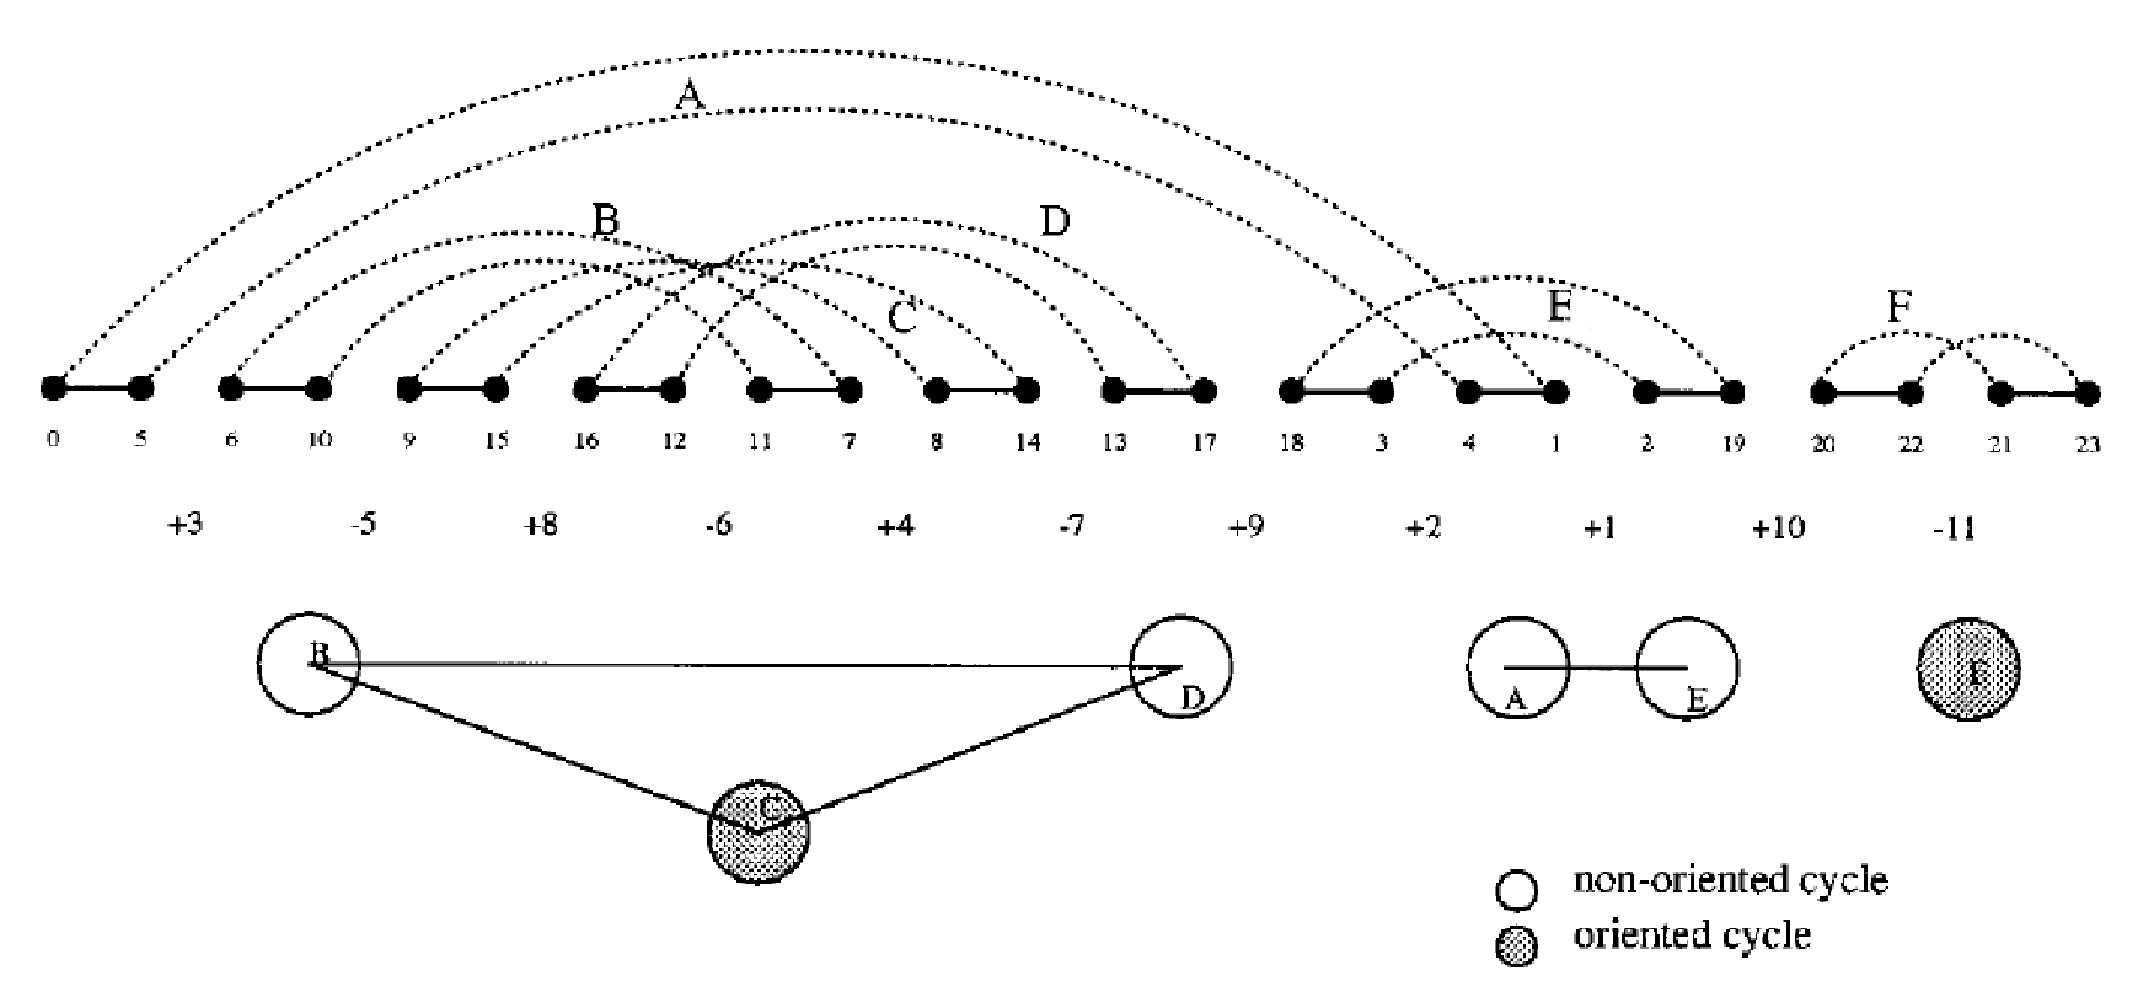
\includegraphics[scale=0.35]{resources/figure_2_c_d.eps}
\caption{Interleaving breakpoint graph $H_{\pi}$ with two oriented and one
unoriented components: black edges connect adjacent vertices that are not
consecutive, gray edges connect consecutive vertices that are not adjacent.
\cite{Hannenhalli95transformingcabbage}}
\label{fig:orientedEdges}
\end{figure}

\paragraph{Oriented and Unoriented Edges} A gray edge \emph{g} is
\textit{oriented} if a reversal acting on two black edges incident to \emph{g}
is proper and \textit{unoriented}, otherwise. 

\paragraph{Example} A gray edge (8, 9) in Figure ~\ref{fig:orientedEdges} is
oriented (since a reversal acting on black edges (8, 14) and (9, 15) destroys
two breakpoints and one cycle) while a gray edge (4, 5) is unoriented. To
provide an intuition for the notion of an oriented edge, we state the following
lemma:

\paragraph{Lemma 1} \textit{Let $(\pi_i, \pi_j)$ be a gray edge incident to
black edges $(\pi_k, \pi_i)$ and $(\pi_j, \pi_l)$. Then $(\pi_i, \pi_j)$
is oriented iff $i - k = j - l$} \cite{Hannenhalli95transformingcabbage}.

\begin{figure}[here]
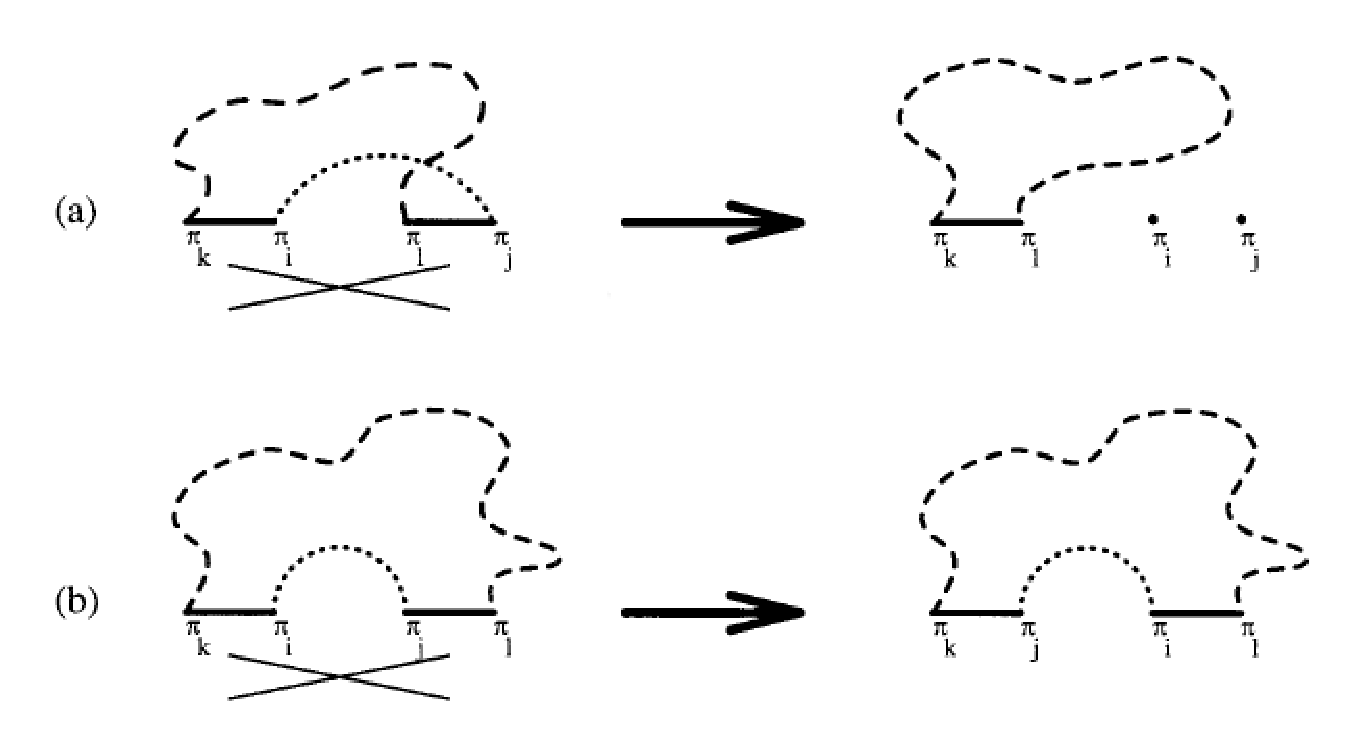
\includegraphics[scale=0.6]{resources/figure_3.eps}
\caption{\cite{Hannenhalli95transformingcabbage}}
\label{fig:figure3}
\end{figure}

\paragraph{Proof} Notice that $k = i \pm 1$ and $l = j \pm 1$. If $i - k = j -
l$, then either $k = i - 1$, $l = j - 1$ or $k = i + 1$, $l = j + 1$ (Figure
~\ref{fig:figure3}(a)). Clearly $\Delta(b - c) = -1$, hence, the reversal acting
on $(\pi_i, \pi_j)$ is proper. If $i - k \neq j - l$, then either $k = i - 1$,
$l = j + 1$ or $k = i + 1$, $l = j - 1$ (Figure ~\ref{fig:figure3}(b)). In this
case, $\Delta(b) = 0$ and $\Delta(c) = 0$; hence, the reversal acting on
$(\pi_i, \pi_j)$ is not proper \cite{Hannenhalli95transformingcabbage}.

\paragraph{Oriented and Unoriented Cycles} A cycle in $G(\pi)$ is
\textit{oriented} if it has an oriented gray edge and \emph{unoriented},
otheriwse. 

\paragraph{Example} Cycles C and F in Figure ~\ref{fig:orientedEdges} are
oriented while cycles A, B, D, and E are unoriented. Clearly, there is no
proper reversal acting on an unoriented cycle. It is esay to see that a
permutation has a proper reversal iff it has an oriented cycle
\cite{Hannenhalli95transformingcabbage}.

\subsection*{Interleaving Edges and Cycles}
Grady edges ($\pi$$_{i}$, $\pi$$_{j}$) and ($\pi$$_{k}$, $\pi$$_{t}$) in
G($\pi$) are interleaving if the intervals $[i, j]$ and $[k, t]$ overlap, but
neither of them contains the other. For example, edges (4,5) and (18,19) in
Figure ~\ref{fig:orientedEdges} are interleaving while edges (4, 5) and (22,
23) are noninterleaving. Two cycles \emph{C$_{1}$} and \emph{C$_{2}$} are
interleaving if there exist interleaving gray edges g$_{1}$ $\in$
\emph{C$_{1}$} and g$_{2}$ $\in$ \emph{C$_{2}$}
\cite{Hannenhalli95transformingcabbage}.

\subsection*{Hurdles and Fortresses}
In breakpoint graphs, \emph{hurdles} present obstacles in the gnome
rearrangement problem. Each additional \emph{hurdle} increases the number of
required reversals (the removal of breakpoints) for a given permutation $\pi$
when transforming into the identity permutation. By considering \emph{hurdles}
in our computations we tighten the bound on the reversal distance problem (see
Calculating the Reversal Distance).

\paragraph{Hurdle} An unoriented cycle component that does \emph{not} seperate
two other unoriented cycle components \cite{1375Algo}.

\paragraph{Simple Hurdle} Not a \emph{Super Hurdle} (see Super Hurdle).

\paragraph{Super Hurdle} A hurdle which protects a non-hurdle from being a
hurdle itself. Deleting a \emph{Super Hurdle} would case the protected
non-hurdle to become a hurdle \cite{Hannenhalli95transformingcabbage}.

\begin{figure}[here!]
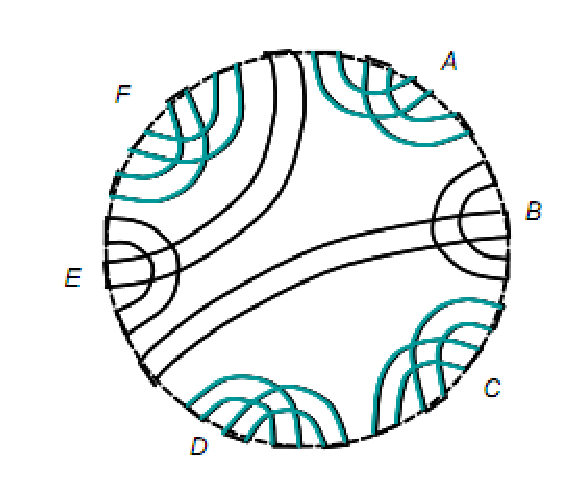
\includegraphics[scale=0.5]{resources/hurdles.eps}
\caption{Simple and Super Hurdles \cite{Hurdles}. Cycles A and F are both super
hurdles becuase they protect cycles B and E (respectively) from becoming
hurdles. While cycles D and C are both simple hurdles.}
\label{fig:hurdles}
\end{figure}

\paragraph{Fortress} A breakpoint graph with an odd number of hurdles which are
\emph{all} \emph{Super Hurdles} \cite{Hannenhalli95transformingcabbage}.

\begin{figure}[here!]
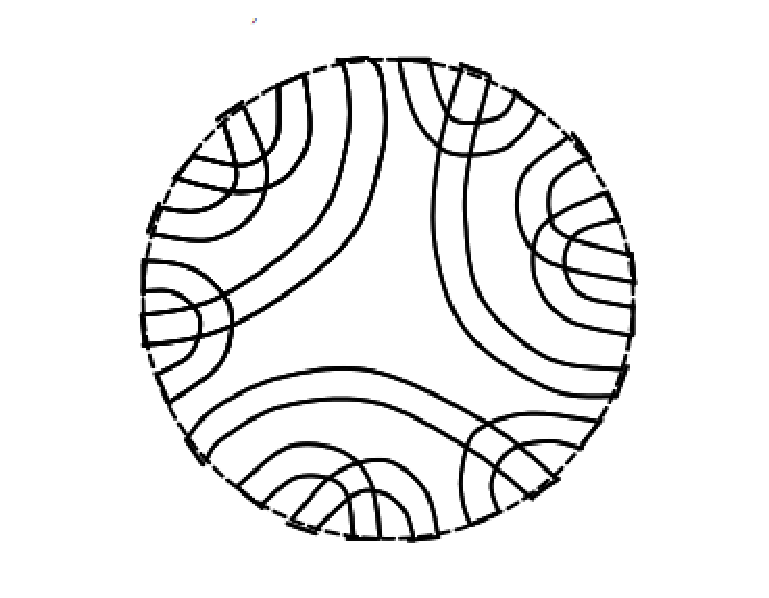
\includegraphics[scale=0.4]{resources/fortresses.eps}
\caption{A 3-Fortress \cite{Hurdles}}
\label{fig:fortresses}
\end{figure}

\subsection*{Calculating the Reversal Distance}

\begin{figure}[here!]
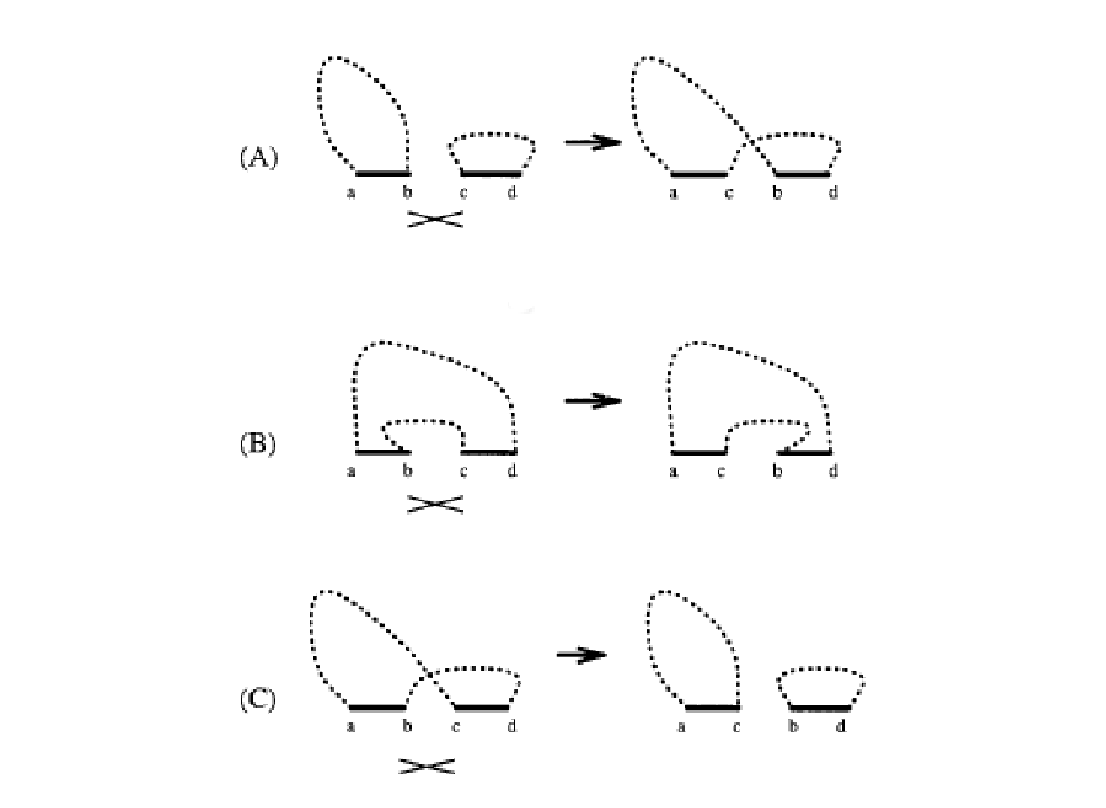
\includegraphics[scale=0.6]{resources/reversals.eps}
\caption{(a) For reversals acting on two cycles, $\Delta$(b - c) = 1.
(b) For reversals acting on an unoriented cycles, $\Delta$(b - c) = 0.
(c) For reversals acting on an oriented cycles, $\Delta$(b - c) = -1.}
\label{fig:reversals}
\end{figure}

\subsubsection*{Theorem 1}
Bafna and Pevzner proved that $\Delta$(b-c) $\in$\{-1, 0, 1\}. 
\\*
\\*
(a) If $\Delta$(b -
c) = 1, then $\Delta$(b - c + h) $\geq$ -1 since $\Delta$h $\geq$ -2 for every
reversal $\rho$
\\*
\\*
(b) If $\Delta$(b-c) = 0,
then $\rho$ acts on a cycle and therefore it affects at most one hurdle. It
implies $\Delta$h $\geq$ -1 and $\Delta$(b - c + h) $\geq$ -1
\\*
\\*
(c) If $\Delta$(b - c)
= -1, then $\rho$ acts on an oriented cycle and hence it does not destroy any
hurdles in $\pi$. Therefore, $\Delta$h $\geq$ 0 and $\Delta$(b - c + h)
$\equiv$ $\Delta$b - $\Delta$c + $\Delta$h $\geq$ -1

Therefore, for an arbitrary reversal $\rho$, $\Delta$(b - c + h) $\geq$ - 1
thus implying d($\pi$) $\geq$ b($\pi$) - c($\pi$) + h($\pi$) \cite{Hannenhalli95transformingcabbage}.

\paragraph{Safe Reversals} A reversal which does \emph{not} create more hurdles
or new unoriented components. A reversal $\rho$ is a safe reversal if
$$\Delta(b - c + h) = -1$$

\subsection*{Equivalent Transformations of Permutations}
Previous studies have revealed that the complicated interleaving structure of
long cycles in breakpoint graphs poses serious difficulties in analyzing
sorting by reversals and transpositions.
\\*
\\*
To get around this problem, we introduce equivalent transformations of
permutations. If a permutation $\pi \equiv \pi(0)$ has a long cycle, transform
it into a new permutation $\pi(1)$ by ``breaking" this long cycle into two
smaller cycles. Continue with $\pi(1)$ in the same manner until you have
filtered out all the long cycles \cite{Hannenhalli95transformingcabbage}.
\\*
\\*
In order to accomplish this task of ``breaking" long cycles, we introduce the
notion of (g, b)-splits and padding.

\begin{figure}[here]
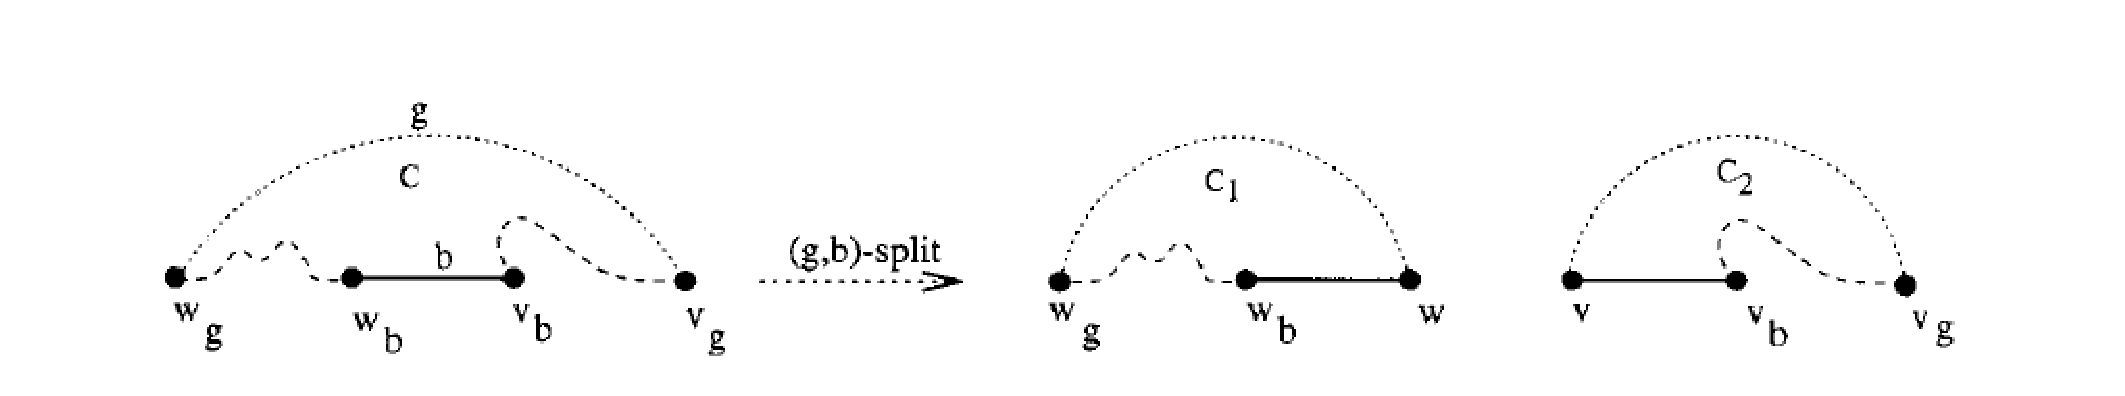
\includegraphics[scale=0.4]{resources/splits.eps}
\caption{Example of a (g, b)-split.}
\label{fig:splits}
\end{figure}

Let b = (v$_{b}$, w$_{b}$) be a black edge and g = (w$_{g}$, v$_{g}$) be a gray
edge belonging to a cycle C = ..., v$_{b}$, w$_{b}$, ..., w$_{g}$, v$_{g}$, ...
in the breakpoint graph G($\pi$) of a permutation $\pi$. A (g, b)-split is a
new graph G'($\pi$) obtained from G($\pi$) by:

\begin{itemize}
    \item Removing edges g and b,
    \item Adding two new vertices v and w,
    \item Adding two new black edges (v$_{b}$, v) and (w, w$_{b}$),
    \item Adding two new gray edges (w$_{g}$, w) and (v, v$_{g}$)
    \cite{Hannenhalli95transformingcabbage}
\end{itemize}

Figure ~\ref{fig:splits} shows a (g, b)-split transforming a cycle C in
G($\pi$) into cycles \emph{C$_{1}$} and \emph{C$_{2}$} in G'($\pi$).

By inducing a (g, b)-split into our graph, we have created what is known as (g,
b) padding.

\begin{figure}[here]
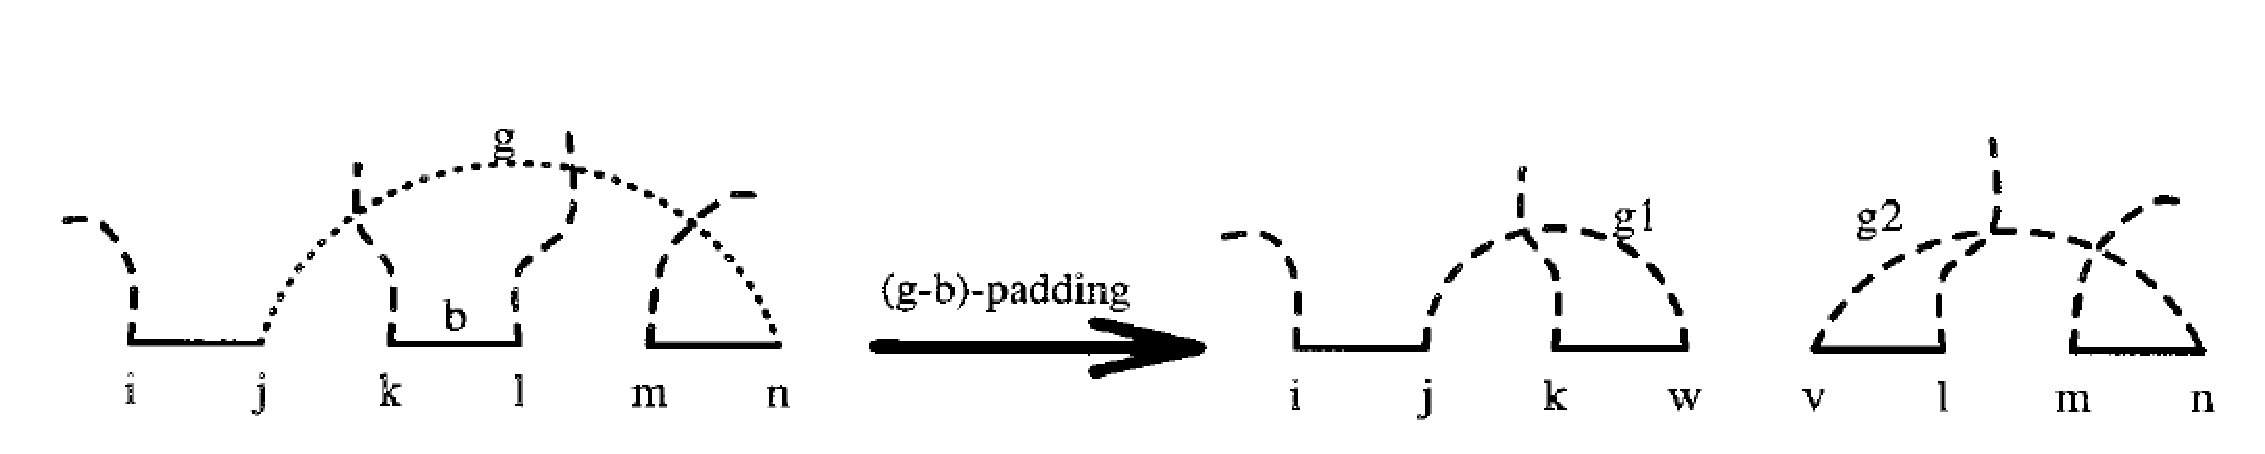
\includegraphics[scale=0.4]{resources/padding.eps}
\caption{A (g, b)-padding deletes an oriented edge g and adds an oriented edge
g$_{1}$ and unoriented edge g$_{2}$}
\label{fig:padding}
\end{figure}

Let b = ($\pi$$_{i+1}$, $\pi$$_{i}$) be a black edge and g = ($\pi$$_{j}$,
$\pi$$_{k}$) be a gray edge belonging to a cycle C = ..., $\pi$$_{i+1}$,
$\pi$$_{i}$, ..., $\pi$$_{j}$, $\pi$$_{k}$, ... in the breakpoint graph
G($\pi$). Define $\Delta$ = $\pi$$_{j}$ - $\pi$$_{k}$, and let v = $\pi$$_{j}$
+ ($\Delta$/3), let w = $\pi$$_{k}$ + ($\Delta$/3). A (g, b)-padding of $\pi$ =
($\pi$$_{1}$$\pi$$_{2}$  ... $\pi$$_{i}$  v w  $\pi$$_{i+1}$ ... $\pi$$_{n}$)
is a permutation of n + 2 elements obtained from $\pi$ by inserting v and w
after the i$^{th}$ element of $\pi (0 \leq i \leq n)$:
$$\pi' = (\pi_{1}\pi_{2}...\pi_{i}vw\pi_{i+1} ... \pi_{n}). $$

Note that v and w are both consecutive and adjacent in $\pi'$. The (g, b)-split
of Figure ~\ref{fig:splits} corresponds to (g, b)-padding for g = (w$_{g}$,
v$_{g}$) and b = (v$_{b}$, w$_{b}$) \cite{Hannenhalli95transformingcabbage}.

\subsection*{Reversal Sort Polynomial Algorithm}

\fbox{
\begin{minipage}{15cm}
\textsc{Algorithm} \textsf{Reversal\_Sort($\pi$)}\\
\textbf{begin}\\
$\mbox{ }\mbox{ }$ \textbf{while} \textsf{$\pi$} is not sorted\\
$\mbox{ }\mbox{ }\mbox{ }\mbox{ }$ \textbf{if} $\pi$ has a long cycle \textbf{then}\\
$\mbox{ }\mbox{ }\mbox{ }\mbox{ }\mbox{ }$ select a safe $(g, b)-$padding $\rho$ of $\pi$\\ 
$\mbox{ }\mbox{ }\mbox{ }\mbox{ }$ \textbf{else if} $\pi$ has an oriented component \textbf{then}\\
$\mbox{ }\mbox{ }\mbox{ }\mbox{ }\mbox{ }$ select a safe reversal $\rho$ in this component\\
$\mbox{ }\mbox{ }\mbox{ }\mbox{ }$ \textbf{else if} $\pi$ has an even number of hurdles \textbf{then}\\
$\mbox{ }\mbox{ }\mbox{ }\mbox{ }\mbox{ }$ select a safe reversal $\rho$ merging two hurdles in $\pi$\\
$\mbox{ }\mbox{ }\mbox{ }\mbox{ }$ \textbf{else if} $\pi$ has at least one simple hurdle \textbf{then}\\
$\mbox{ }\mbox{ }\mbox{ }\mbox{ }\mbox{ }$ select a safe reversal $\rho$ cutting this hurdle in $\pi$\\
$\mbox{ }\mbox{ }\mbox{ }\mbox{ }$ \textbf{else if} $\pi$ is a fortress with more than three superhurdles \textbf{then}\\
$\mbox{ }\mbox{ }\mbox{ }\mbox{ }\mbox{ }$ select a safe reversal $\rho$ merging two (super)hurdles in $\pi$\\
$\mbox{ }\mbox{ }\mbox{ }\mbox{ }$ \textbf{else} /* $\pi$ is a 3-fortress */\\
$\mbox{ }\mbox{ }\mbox{ }\mbox{ }\mbox{ }$ select an (un)safe reversal $\rho$ merging two arbitrary (super)hurdles in $\pi$\\
$\mbox{ }\mbox{ }\mbox{ }$ $\pi \leftarrow \pi \dot{ } \rho$\\
$\mbox{ }\mbox{ }$\textbf{end while}\\
\textbf{end}\\
\end{minipage}
}

\subsection*{Example Run of Reversal Sort Algorithm}
Using the predefined set of permutations in Figure ~\ref{fig:orientedEdges}, we will trace through the reversal sort
algorithm.

\subsubsection*{Step 1 - $\pi$ has an oriented component}
$[0, 5, 6, 10, 9, \textbf{15, 16, 12, 11, 7, 8}, 14, 13, 17, 18, 3, 4, 1, 2, 19, 20, 22, 21, 23]$
\\*
\\*
Cycles :\\(0, 1, 4, 5, 0) - Simple Hurdle, 
        \\(6, 7, 11, 10, 6) - Simple Hurdle, 
        \\(9, 8, 14, 15, 9) - Oriented Cycle, 
        \\(18, 19, 2, 3, 18) - Simple Hurdle, 
        \\(16, 17, 13, 12, 16) - Simple Hurdle,
        \\ (20, 21, 23, 22, 20) - Oriented Cycle
\\*
\\*
Reversal: \textbf{15, 16, 12, 11, 7, 8} $\rightarrow$ \textbf{8, 7, 11, 12, 16, 15}
\subsubsection*{Step 2 - $\pi$ has an oriented component}
$[0, 5, 6, 10, 9, 8, 7, 11, 12, 16, 15, 14, 13, 17, 18, 3, 4, 1, 2, 19, 20, \textbf{22, 21}, 23]$
\\*
\\*
Cycles :\\(0, 1, 4, 5, 6) - Simple Hurdle,
        \\(6, 7, 11, 10, 6) - Oriented Cycle,
        \\(12, 13, 17, 16, 12) - Oriented Cycle,
        \\(18, 19, 2, 3, 18) - Simple Hurdle
\\*
\\*
Reversal: \textbf{22, 21} $\rightarrow$ \textbf{21, 22}

\subsubsection*{Step 3 - $\pi$ has an oriented component}
$[0, 5, 6, \textbf{10, 9, 8, 7}, 11, 12, 16, 15, 14, 13, 17, 18, 3, 4, 1, 2, 19, 20, 21, 22, 23]$
\\*
\\*
Cycles :\\(0, 1, 4, 5, 0) - Simple Hurdle,
        \\(6, 7, 11, 10, 6) - Oriented Cycle,
        \\(12, 13, 17, 16, 12) - Oriented Cycle,
        \\(18, 19, 2, 3, 18) - Simple Hurdle
\\*
\\*
Reversal: \textbf{10, 9, 8, 7} $\rightarrow$ \textbf{7, 8, 9, 10}

\subsubsection*{Step 4 - $\pi$ has an oriented component}
$[0, 5, 6, 7, 8, 9, 10, 11, 12, \textbf{16, 15, 14, 13,} 17, 18, 3, 4, 1, 2, 19, 20, 21, 22, 23]$
\\*
\\*
Cycles :\\(0, 1, 4, 5, 0) - Simple Hurdle,
        \\(12, 13, 17, 16, 12) - Oriented Cycle,
        \\(18, 19, 2, 3, 18) - Simple Hurdle
\\*
\\* 
Reversal: \textbf{16, 15, 14, 13} $\rightarrow$ \textbf{13, 14, 15, 16}
\subsubsection*{Step 5 - $\pi$ has an oriented component}
$[0, 5, 6, 7, 8, 9, 10, 11, 12, 13, 14, 15, 16, 17, 18, \textbf{3, 4, 1, 2, 19}, 20, 21, 22, 23]$
\\*
\\*
Cycles :\\(0, 1, 4, 5, 0) - Simple Hurdle,
        \\(18, 19, 2, 3, 18) - Simple Hurdle
\\*
\\*
Reversal: \textbf{3, 4, 1, 2, 19} $\rightarrow$ \textbf{19, 2, 1, 4, 3}
\subsubsection*{Step 6 - $\pi$ has an even number of hurdles}
$[0, \textbf{5, 6, 7, 8, 9, 10, 11, 12, 13, 14, 15, 16, 17, 18, 19, 2, 1}, 4, 3, 20, 21, 22, 23]$
\\*
\\*
Cycles :\\(0, 1, 4, 5, 0) - Oriented Cycle,
        \\(19, 20, 3, 2, 19) - Simple Hurdle
\\*
\\*
Reversal: \textbf{5, 6, 7, 8, 9, 10, 11, 12, 13, 14, 15, 16, 17, 18, 19, 2, 1} $\rightarrow$
\\* \textbf{1, 2, 19, 18, 17, 16, 15, 14, 13, 12, 11, 10, 9, 8, 7, 6, 5}
\subsubsection*{Step 7 - $\pi$ has an oriented component}
$[0, 1, 2, \textbf{19, 18, 17, 16, 15, 14, 13, 12, 11, 10, 9, 8, 7, 6, 5, 4, 3}, 20, 21, 22, 23]$
\\*
\\*
Cycles :\\(2, 3, 20, 19, 2) - Oriented Cycle
\\*
\\*
Reversal: \textbf{19, 18, 17, 16, 15, 14, 13, 12, 11, 10, 9, 8, 7, 6, 5, 4, 3} $\rightarrow$
\\* \textbf{3, 4, 5, 6, 7, 8, 9, 10, 11, 12, 13, 14, 15, 16, 17, 18, 19}
\subsubsection*{Step 8 - $\pi$ is sorted}
$[0, 1, 2, 3, 4, 5, 6, 7, 8, 9, 10, 11, 12, 13, 14, 15, 16, 17, 18, 19, 20, 21, 22, 23]$

\nocite{*}
\bibliographystyle{IEEEannot}
\bibliography{biblio}

\end{document}
